\documentclass[12pt]{report}
\usepackage[utf8]{inputenc}
\usepackage[romanian]{babel}
\usepackage{graphicx}
\usepackage[a4paper,left=30mm,right=20mm,top=25mm,bottom=25mm,bindingoffset=6mm]{geometry}
\usepackage[nottoc]{tocbibind}
\usepackage{subcaption}
\usepackage{listings}
\usepackage{amsfonts}
\usepackage{amsmath}
\usepackage{adjustbox}
\setlength{\parindent}{2em}
\setlength{\parskip}{0,7em}
\renewcommand{\baselinestretch}{1.5}

\usepackage{fancyhdr}
\fancyhead{}
\fancyhead[RO,LE]{\leftmark}
\fancyfoot{}
\fancyfoot[LE,RO]{\thepage}
%\fancyfoot[LO,CE]{Capitolul \thechapter}
%\fancyfoot[CO,RE]{Ionut N. Ciocoiu}
\renewcommand{\headrulewidth}{0.4pt}
\renewcommand{\footrulewidth}{0.4pt}
\pagestyle{fancy}

\graphicspath{ {imagini/} }

\usepackage{color}   %May be necessary if you want to color links
\usepackage{hyperref}
\hypersetup{
	colorlinks=true, %set true if you want colored links
	linktoc=all,     %set to all if you want both sections and subsections linked
	linkcolor=blue,  %choose some color if you want links to stand out
}

\newcommand\tab[1][1cm]{\hspace*{#1}}

%\usepackage{natbib}
\usepackage[square,numbers]{natbib}
%\bibliographystyle{abbrvnat}
\bibliographystyle{unsrtnat}
%\setcitestyle{numbers, authoryear,open={(},close={)}}

\hyphenation{Numpy}

\newtheorem{teo}{Teorema}[chapter]
\newtheorem{lema}[teo]{Lema}
\newtheorem{dfn}[teo]{Definiția}
\newtheorem{cor}[teo]{Corolar}
\newtheorem{prop}[teo]{Propoziția}
\newtheorem{obs}[teo]{Observația} 
\newtheorem{exm}[teo]{Exemplu}

\usepackage{listings}

\definecolor{cred}{RGB}{230,25,60}
\definecolor{cgreen}{RGB}{41,163,41}
\definecolor{cmagenta}{RGB}{230,25,195}
\definecolor{cviolet}{RGB}{173,43,238}
\definecolor{corange}{RGB}{135,113,29}
\definecolor{cyellow}{RGB}{152,152,27}
\definecolor{cblue}{RGB}{61,98,245}
\definecolor{backcolour}{RGB}{244, 251, 244}

\lstdefinestyle{mystyle}{
	backgroundcolor=\color{backcolour},   
	commentstyle=\color{cgreen},
	keywordstyle=\color{cblue},
	numberstyle=\tiny\color{corange},
	stringstyle=\color{cmagenta},
	basicstyle=\footnotesize,
	breakatwhitespace=false,         
	breaklines=true,                 
	captionpos=b,                    
	keepspaces=true,                 
	numbers=left,                    
	numbersep=10pt,                  
	showspaces=false,                
	showstringspaces=false,
	showtabs=false,                  
	tabsize=4
}

\lstset{style=mystyle}

\renewcommand{\lstlistlistingname}{Lista porțiunilor de cod}
\begin{document}
	\begin{titlepage}
	
	\newcommand{\HRule}{\rule{\linewidth}{0.5mm}} % Defines a new command for the horizontal lines, change thickness here
	
	\center % Center everything on the page
	
	%----------------------------------------------------------------------------------------
	%	HEADING SECTIONS
	%----------------------------------------------------------------------------------------
	
	\textsc{\LARGE UNIVERSITATEA DIN BUCUREȘTI}\\[1.5cm] % Name of your university/college
	\textsc{\Large FACULTATEA DE MATEMATICĂ ȘI INFORMATICĂ}\\[0.5cm] % Major heading such as course name
	\textsc{\large LUCRARE DE DISERTAȚIE}\\[0.5cm] % Minor heading such as course title
	
	%----------------------------------------------------------------------------------------
	%	TITLE SECTION
	%----------------------------------------------------------------------------------------
	
	\HRule \\[0.4cm]
	{ \huge \bfseries Agent conversațional}\\[0.4cm] % Title of your document
	\HRule \\[1.5cm]
	
	%----------------------------------------------------------------------------------------
	%	AUTHOR SECTION
	%----------------------------------------------------------------------------------------
	
	\begin{minipage}{0.4\textwidth}
		\begin{flushleft} \large
			\emph{Student:}\\
			Ionuț Ciocoiu % Your name
		\end{flushleft}
	\end{minipage}
	~
	\begin{minipage}{0.4\textwidth}
		\begin{flushright} \large
			\emph{Coordonator științific:} \\
			Prof. Dr. Liviu P. Dinu % Supervisor's Name
		\end{flushright}
	\end{minipage}\\[4cm]
	
	% If you don't want a supervisor, uncomment the two lines below and remove the section above
	%\Large \emph{Author:}\\
	%John \textsc{Smith}\\[3cm] % Your name
	
	
	%	LOGO SECTION
	%----------------------------------------------------------------------------------------
	
	
\includegraphics[scale=0.3]{fmi_logo.jpg}\\[1cm] % Include a department/university logo - this will require the graphicx package
	
	%----------------------------------------------------------------------------------------
	%----------------------------------------------------------------------------------------
	%	DATE SECTION
	%----------------------------------------------------------------------------------------
	\vfill % Fill the rest of the page with whitespace
	{\large FEBRUARIE 2019}\\[3cm] % Date, change the \today to a set date if you want to be precise
	
	%----------------------------------------------------------------------------------------
	
\end{titlepage}
	%\chapter*{Abstract}
	%Abstract goes here
	
	%\chapter*{Dedication}
	%To mum and dad
	
	%\chapter*{Declaration}
	%I declare that..
	
	%\chapter*{Acknowledgements}
	%I want to thank...
	
	\tableofcontents
	
	\listoffigures

	%\listoftables
	
	\lstlistoflistings
	
	\chapter{Introducere}

Dincolo de utilitatea practică de a transmite informații, limbajul este cel care intensifică interacțiunea și menține legăturile interumane. Făcând o paralelă cu sintagma "o imagine valorează cât o mie de cuvinte" la fel un proverb românesc surprinde esența cu: \textit{"Vorba dulce mult aduce"}, reliefând astfel caracterul artistic și contemplativ, trăsătură pusă într-o antiteză chiar de caracterul pragmatic din debut. Cu alte cuvinte limbajul este uneori paradoxal, iar cuvintele ar putea curge la nesfârșit spre deslușirea acestei capacități,

În cartea sa Speach Proccessing, profesorul Dan Jurafski observă faptul că există numeroase exemple în care omul încearcă să comunice cu creația sa, acest comportament este surprins adesea și în literatură unde personificarea nu se oprește numai la natură. Această remarcă arată de fapt longevitatea și neoboseala dorinței creatoare concretizată chiar în această ramură a lingvisticii matematice care ne permite cu adevărat să dăm naștere unui astfel de agent conversațional.

\section{Motivația}

Luând contact tot mai des cu mediul de cercetare, încerc să observ modul în care această comunitate reușește să aducă contribuții în societate. Un lucru care m-a făcut sa prețuiesc fiecare efort, este acela că în general o descoperire se bazează pe cercetări anterioare și ca orice gând exprimat în scopul de a descoperi, poate fi valoros și dus mai departe spre cunoaștere.

Dorința de a crea cu scopul de face viața oamenilor mai ușoară este imboldul intrinsec ce ghidează acțiunile mele, așadar evaluând cunoștințele mele, am decis sa îmi aduc contribuția într-un domeniu atât de important în drumul nostru spre o viziune clara.

\section{Descrierea problemei}

Lucrarea își propune descoperirea unui model îndeajuns de puternic încât să înțeleagă limbajul natural exprimat într-un anumit context (general sau specific unui domeniu). Și punerea în aplicare a unui administrator de dialog, suficient de simplu dar care să ducă la bun sfărșit sarcinile dorite spre a fi executate de care agentul virtual rezultat.

În viziunea mea, această chestiune reprezintă mai degrabă o nevoie decât o problemă. O nevoie ce survine în urma stilului nostru de viață dinamic și învelit în straturi de informație.

Cum limbajul natural este cel mai la îndemâna instrument de comunicare, consider ca prin intermediul său vom putea satisface nevoia unei interfețe capabile să ușureze interacțiunea dintre noi și tehnologie.

\section{Progres precedent}
Mergând pe acest drum al construirii unui sistem de dialog în literatura de specialitate se disting două ramuri: cea a asistenților digitali care rezolvă diferite cerințe, în general conversația nu este menită dă dureze mult, iar rolul agentului este de a capta informații din conversația cu utilizatorul și de a-l ajuta să ducă la bun sfârșit o operație \cite{Tasc_oriented}. În cea de-a doua direcție este vorba despre agenți conversaționali (chatbots), acest termen face referire la un agent orientat spre discuție la nivel general, servind mai de grabă unui scop subiectiv decât unuia obiectiv soluțional. În această situație dialogul poate dura mai mult, existând și aplicații practice ale acestuia cum ar fi cea de a testa anumite teorii psihologice \cite{weizenbaum}

Pornind de la dorința de a crea cu scopul de a aduce valoare în societate, am ales ca direcție de studiu sistemul de dialog orientat pe rezolvarea cerințelor. Tot mai des se încearcă metode end-to-end pentru a descoperi un singur model care să țină loc unui astfel de sistem \cite{end-to-end foal oriented}. În industrie lucrurile sunt abordate mai modular, antrenându-se modele diferite pentru fiecare componentă (ASR, SLU/NLU, DM, NLG). Un minimum viabil al acestei arhitecturi modulare îl reprezintă componenta de înțelegerea limbajului natural(NLU) și cea de administrare a dialogului (DM) acestea două făcând obiectul lucrării de față.

Componenta de înțelegerea limbajului natural se ocupă cu detectarea intenției și a entităților aflate într-o replică venită din partea utilizatorului. De multe ori cele două chestiuni sunt văzute separat, ca o problemă de clasificare respectiv ca o problemă de etichetare a unei secvențe.
Pentru detectarea intenției se folosesc abordări precum \cite{id_classifiers}. Iar pentru recunoașterea entităților sunt folosite tehnici de etichetare ca \cite{scipy_numpyeq_labeling}. Dar luând în considerare puterea rețelelor neuronal recurente și a arhitecturii de codificare-decodificare utilizată cu succes în traducere și recunoașterea vorbirii \cite{luoung_bahdanau_maning}. Aceste două probleme sunt tratate de multe ori concomitent, în esență se folosește capacitatea de a capta înțelesul unei secvențe de text cu ajutorul unui encoder iar apoi se folosesc diferite decodere pentru a traduce cuvinte sau întregul înțeles în clase de intenții și entități.

Privind comunicarea ca o nevoie de bază ne ajută sa vedem mai clar de ce procesarea limbajului natural este un element esențial in drumul nostru spre cunoaștere. Datorită actualului progres in acest domeniu ne putem bucura de ușurința cu care informațiile circulă între noi, făcând realizabil acest avânt tehnologic de care nu bucurăm cu toții.

% sa spun despre abordari anterioare si referinte la ele, cum m-am gandit eu si experimentat (pe scurt)
% problematica
% contributia mea
% rezumatul capitolelor
% baseline rezultate
% sa scriu despre analiza erorilor cu exemplu, unde greseste




\section{Rezumatul capitolelor}

\begin{description}
	\item[Introducere]  - 
	
	Capitolul întâi vorbește in principal despre modul în care această lucrare își propune să rezolve nevoia de interacțiune cu tehnologia, dar și despre un capitol istoric privit prin ochii unei motivații îndraznețe.
	\item
	Atunci când se rostește "progres" am în minte o  spirală a cunoștintelor care se bazează unele pe altele. Precum această imagine implementarea acestei tehnologi de dialog impune un anumit progres precedent, așa că în capitolul doi vor fi prezentate aceste instrumente care fac posibilă aceasta tehnologie.
	\item
	In capitolul al treilea vor fi explicate modelele matematice care stau în spatele modelelor decizionale.
	\item
	In partea a patra se prezintă modulul de înțelegerea limbajului natural
	\item
	Al cincelea capitol descrie modulul care ține contextul unei conversații.
	\item
	Iar in partea de final concluziile referitoare la studiul elaborat in această teză.
\end{description}


	
	\chapter{Dialog}

Conform definiției din limba română, dialogul este modul de expunere care prezintă succesiunea replicilor dintr-o conversație care are loc între două sau mai multe persoane.

Această lucrare își propune să dea formă înțelegerii limbajului natural dintr-o perspectivă matematică, prezentând sub forma unei soluții programabile un întreg sistem de micro servicii toate funcționând sub umbrela aceluiași scop, comunicarea.

Pe parcursul lucrării se va face referire la dialog ca o secvență de replici între un om și un calculator pentru a transmite informații.
Referitor la componentele unui dialog, se va prezenta doar o abordare bazată pe componenta \textit{verbală}, celelalte componente - \textit{nonverbală} (gesturi, mimică, poziția corpului) și \textit{paraverbală} (accentul, ritmul și intensitatea vorbirii) - făcând obiectul altor lucrări viitoare.


\section{Conversația naturală}

Un factor cheie într-o conversație este acela că fiecare replică dintr-un dialog este o formă de \textbf{acțiune} venită din partea vorbitorului \cite{witt1953}. În literatura de specialitate \textbf{actele de vorbire} sunt cele ce dau tipul acestor acțiuni.

De-a lungul timpului s-au propus numeroase moduri de a grupa acte de vorbire, iar modul de clasificare potrivit abordării de față conține doar 4 categorii și se concentrează pe intenția comunicată, conținutul propozițional și contextul de producere.

\subsection{Acte de vorbire}
\begin{enumerate}
	\item \textbf{Reprezentative (asertive)} - sunt acele acte care definesc o constatare. Cu ajutorul lor se comunică informații se impun constrângeri, iar la nivel de conținut putem spune că descriu realitatea. Se descriu anumite evenimente ("Coletul a fost livrat"), sau se impun anumite constrângeri ("Voi pleca maine"). Mărcile acestui act de vorbire sunt date de verbe precum: \textit{a afirma, a admite, a anunța, a avertiza, a declara, a insista, a înștiința, a zice, etc}.

	\item \textbf{Directive} - sunt actele ce urmăresc impunerea unei acțiuni. Scopul lor este de a determina participanții la dialog să execute o sarcină. Verbele marcante sunt \textit{a întreba, a interzice, a ordona, a cere}
	
	\item \textbf{Expresive} -  reprezintă o manifestare în plan verbal a sentimentelor, emoțiilor și a atitudinilor vorbitorului cu referire la acțunile întreprinse sau nu de către interlocutor. Verbele reprezentative ale acestui act sunt: \textit{a mulțumi, a lăuda, a felicita, a regreta, a reproșa, a critica, a acuza, etc}
	
	\item \textbf{Comisive (promisive)} - vizează angajamentul locutorului de a da curs unor acțiuni/convingeri \textit{a promite, a plănui, a jura, a paria, a se opune}
\end{enumerate}

Pentru stabilirea intenției, actul de vorbire joacă un rol foarte important, iar sistemele de dialog extind aceste clasificări în intenții specifice domeniului cu scopul de a caracteriza cât mai bine conversația.

%todo: Exemplu de intenții si cum sunt ele văzute in administratorul de dialog.

\section{Sistem de dialog}
Conversația cu un robot presupune o înlănțuire de servicii văzută ca un ciclu de informații ce se mulează pe nevoile exprimate de către vorbitor. În continuare sunt prezentate componente care fac posibilă această conexiune.
% todo: de descris fiecare modl ]n parte
\subsection{Componente}
\begin{figure}[h]
	\centering
	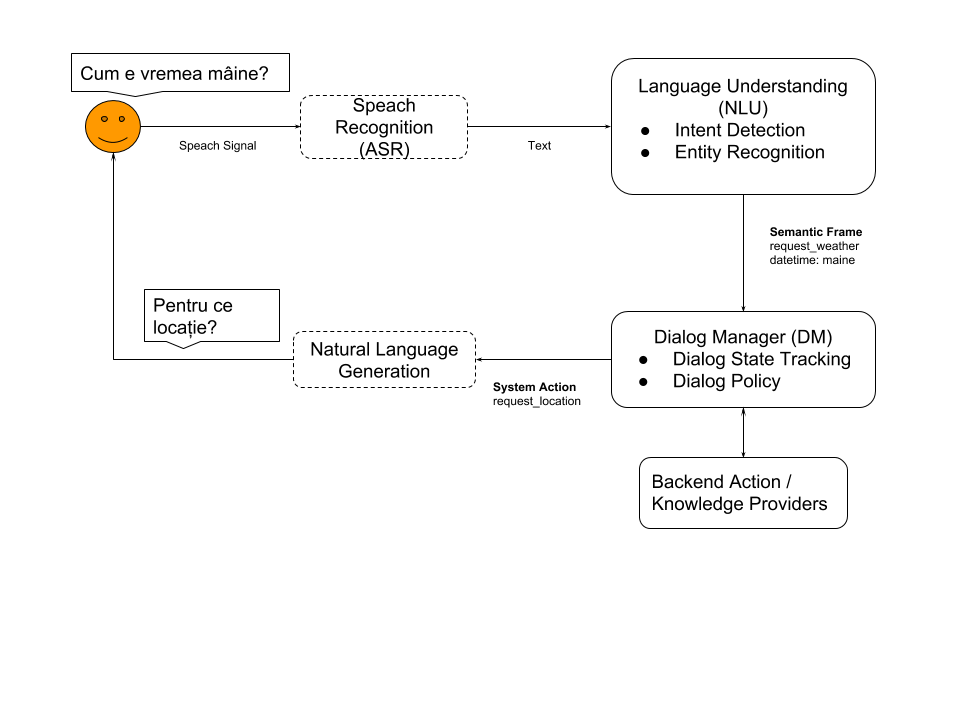
\includegraphics[scale=0.3]{dialog_system.png}
	\caption{Sistem de Dialog Modular}
	\label{fig:ds_proc}
\end{figure}
\begin{description}
	\item[Din voce în text - Speech To Text (STT)]  - 
	Este serviciul care se ocupă cu recunoașterea și conversia în text a semnalelor vocale
	\item[Înțelegerea limbajului natural - Natural Language Understanding (NLU)] -
	Componenta responsabilă de cadrul semantic ce descrie intenția și entitățile menționate de utilizator
	\item[Administrator de dialog - Dialog Manager (DM)] - 
	Este modulul ce gestionează dialogul, având ca funcții principale reprezentarea contextului și inferența pe baza acestuia
	\item[Generarea de limbaj natural - Natural Language Generation (NLG)] -
	După ce administratorul de dialog decide ce acțiune să execute, el o pasează mai departe componentei de generare a limbajului care transformă dintr-o reprezentare internă simplificată într-o replică de dialog
	\item[Din text în voce - Text To Speech] - 
	Ultima procesare este produsă de componenta care generează semnale vocale pe baza textului primit de la NLG
\end{description}

Întregul proces este descris de diagrama din figura \ref{fig:ds_proc}. Totul începe cu utilizatorul care formulează o cerere către sistem, vocea acestuia este procesată de către modulul de recunoaștere vocală care întoarce textul rostit de către vorbitor. Cererea în format text este apoi trimisă la modulul de înțelegere a limbajului care detectează la rându-i, intenția utilizatorului dar și entitățile menționate. Acest cadru semantic extras este apoi trimis modulului care ține firul dialogului și în funcție de definiția sarcinii pe care utilizatorul o dorește a fi îndeplinită se iau acțiunile în consecință și se trimite răspunsul către utilizator.

Doar componenta de înțelegere a limbajului și cea de administrare a dialogului vor fi analizate în cele ce urmează, întrunindu-se astfel minimul necesar unei conversații scrise.
	
	\chapter{Sistem de dialog}

\section{Înțelegerea limbajului natural}

\subsection{Abordări anterioare}

\subsection{Seq2Seq}

\begin{figure}[h]
	\centering
	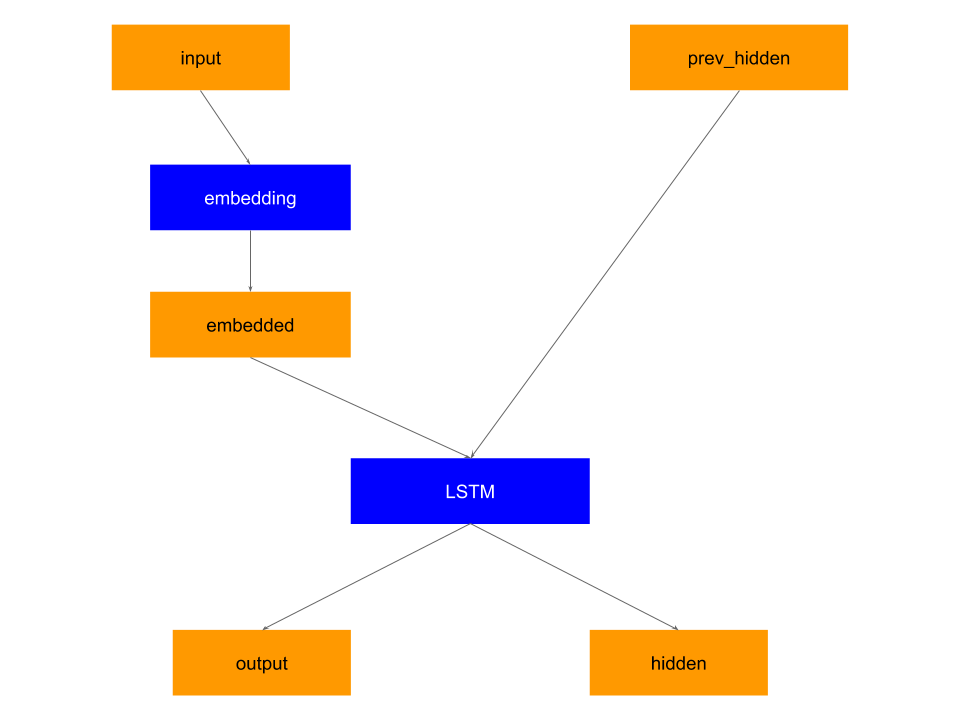
\includegraphics[scale=0.35]{encoder_module.png}
	\caption{Bidirectional Encoder}
	\label{fig:enc_module}
\end{figure}


\begin{figure}[h]
	\centering
	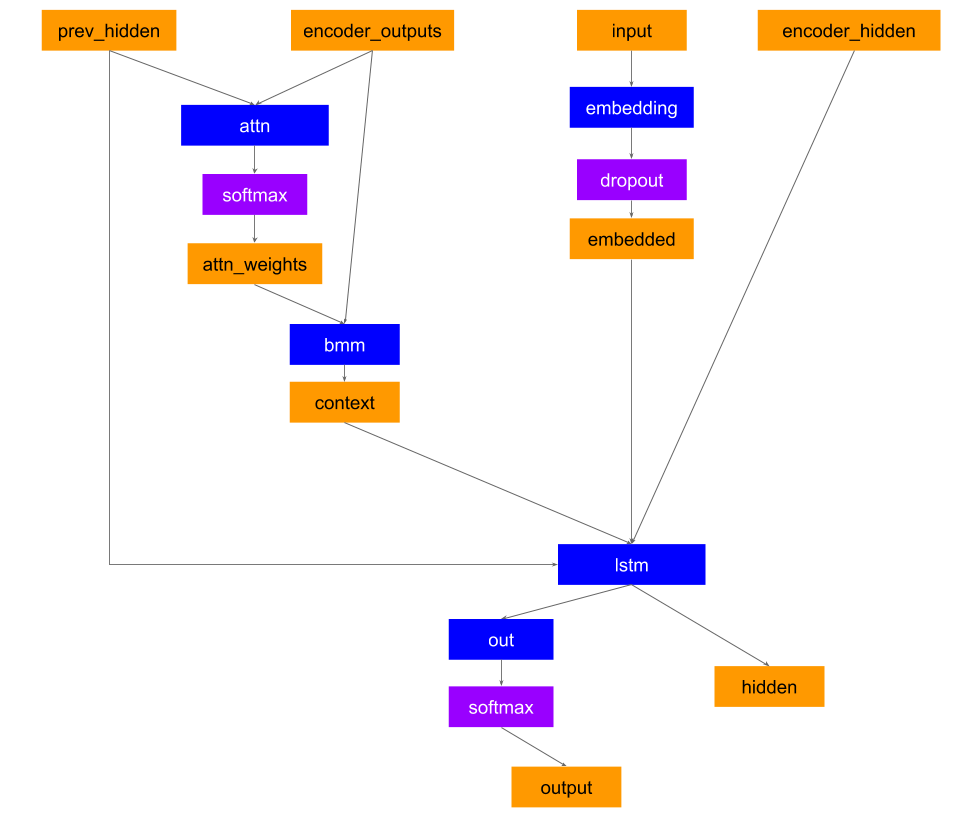
\includegraphics[scale=0.35]{decoder_bahdanau.png}
	\caption{Decoder Bahdanau}
	\label{fig:dec_bah}
\end{figure}

\section{Administrator de dialog}

\subsection{Abordări anterioare}

\subsection{Slot filling}

\section{Metode de evaluare}

\section{Rezultate}
		
	\chapter{Noțiuni teoretice}

\section{Rețele Neurale Recurente}

Rețelele neuronale recurente (RNN - Recurent Neural Networks), sunt o arhitectura aparte de rețele neuronale, ce le face atat de speciale este faptul ca ele reușesc sa capteze secvențialitatea datelor. Ele sunt folosite in special în procesarea limbajului natural, dar și în procesarea imaginilor, a seriilor de timp, a recomandarilor de produse. Cu alte cuvinte oricând vine vorba de succesiunea anumitor evenimente, ele reprezintă un candidat bun în captarea acestor modele in date.

Figura \ref{fig:rnn_arch} prezintă arhitectura unei rețele recurente, unde fiecare dreptunghi ține locul stratului ascuns de la pasul, $t$. Fiecare strat ascuns este format din perceptroni care execută operația de inmulțire intre parametrii și input, urmată de o operație nonlineară (ex.$ tanh$). La fiecare pas din timp, ieșirea de la pasul anterior, împreună cu vectorul următorului cuvânt, $x_t$, sunt intrări în stratul ascuns care produce pentru pasul următor, iețirea $y$, și vectorul de caracteristici al stratului ascuns, $h$.


\begin{equation}
	h_t = \sigma{(W^{(hh)} h_{t-1} + W^{(hx)} x_{[t]})}
	\label{h_t}
\end{equation}

\begin{equation}
	y_t = softmax(W^{(S)} h_t) 
	\label{y_t}
\end{equation}

\begin{figure}[h]
	\centering
	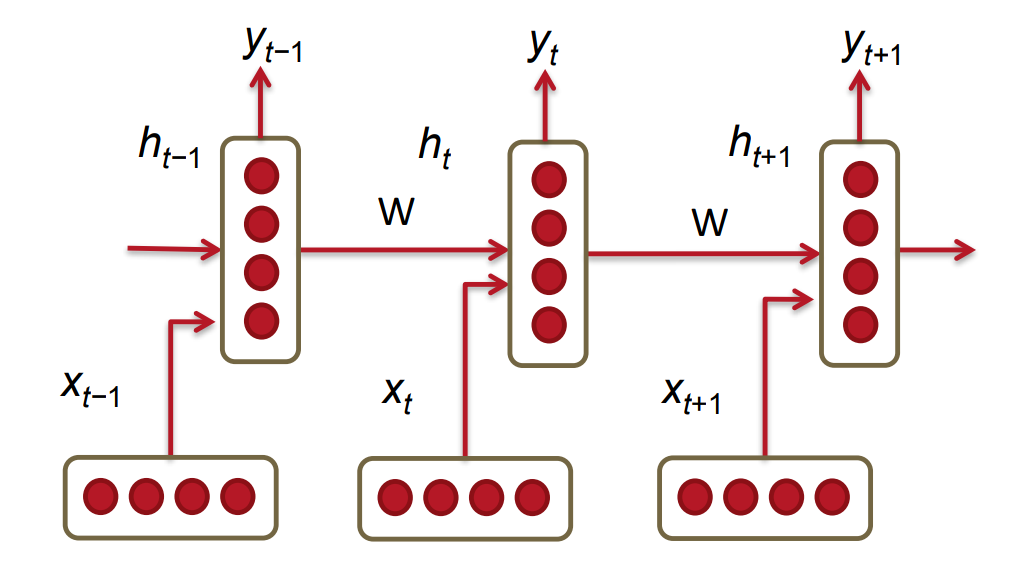
\includegraphics[scale=0.3]{rnn_arch.png}
	\caption{Arhitectura RNN \cite{cs224d_notes}}
	\label{fig:rnn_arch}
\end{figure}

Descrierea parametrilor din rețea:

\begin{itemize}
	\item $x_1, x_2, ..., x_T$ vectorii cuvintelor dintr-o secvență de lungime $T$
	\item $h_t = \sigma{(W^{(hh)} h_{t-1} + W^{(hx)} x_{[t]})}$: formula care descrie calculul vectorului de caracteristici, $h_t$, la fiecare pas $t$:
	
	\begin{itemize}
		\item $ x_t \in {\rm I\!R}^d $ vectorul cuvântului $t$
		\item $ W^{hx} \in {\rm I\!R}^{D_h \times d} $ matricea proderilor utilizată la condiționarea vectorului de intrare, $x_t$
		\item $ W^{hh} \in {\rm I\!R}^{D_h \times D_h} $ matricea proderilor utilizată la condiționarea ieșirii de la pasul anterior, $h_{t-1}$
		\item $ h_{t-1} \in  {\rm I\!R}^{D_h} $ ieșirea funcției nonlineare de la pasul anterior, $t-1$, iar $h_0 \in  {\rm I\!R}^{D_h}$ este vectorul de inițializare pentru stratul ascuns, la pasul $t=0$
		\item $ \sigma() $ funcția nonlineară  (sigmoid in acest exemplu)
	\end{itemize}

	\item $ y_t = softmax(W^{(S)} h_t) $ ieșirea care reprezintă o distribuție de probabilitate peste vocabular la fiecare pas $t$. În esență, $y_t$ este următorul cuvânt prezis, dându-se contextul de până  acum ($ h_{t-1} $) și ultimul cuvânt observat ($x_t$). Avem  $ W^{S} \in {\rm I\!R}^{|V| \times D_h} $ și $ y \in {\rm I\!R}^{|V|} $, unde $|V|$ reprezintă cardinalitatea mulțimii $V$ adică a vocabularului de cuvinte.

\end{itemize}

Funcția de cost utilizată in rețelele neuronale recurente este de obicei CE (cross entropy error).

Pentru pasul $t$:
$$
J_{(t)}(\theta) = - \sum_{j=1}^{|V|}  ytrue_{t, j} \times \log(y_{t, j})
$$

% todo sa investighez de ce nu dispare minusul, eroare in formula
Pentru toată secvența de lungime $T$ funcția de cost devine:
$$
J = - \frac{1}{T} \sum_{t=1}^{T} J_{(t)}(\theta) = - \frac{1}{T} \sum_{t=1}^{T}  \sum_{j=1}^{|V|}  ytrue_{t, j} \times \log(y_{t, j})
$$

\cite{cs224d_notes}


\subsection{Problema dispariției sau a explodării valorilor gradientului}
O RNN împarte aceeași matrice a parametrilor pentru toată secvența de intrare. Țelul unei astfel de arhitecturi este acela de a capta contextul și în cazul secvențelor de lungimi mai mari.

Considerăm ecuațiile \ref{h_t} și \ref{y_t} de mai sus la pasul $t$. Pentru a calcula eroarea unei RNN, $dE/dW$, vom însuma erorile de la fiecare pas de timp.

\begin{equation}
	\frac{\partial E}{\partial W} = \sum_{t=1}^{T} \frac{\partial E_t}{\partial W}
\end{equation}

Eroarea la fiecare pas de timp este calculată prin diferențierea ecuațiilor  \ref{h_t} și \ref{y_t}:

\begin{equation}
	\frac{\partial E_t}{\partial W} = \sum_{k=1}^{t} \frac{\partial E_t}{\partial y_t} \frac{\partial y_t}{\partial h_t} \frac{\partial h_t}{\partial h_k} \frac{\partial h_k}{\partial W}
	\label{chain_rule_E}
\end{equation}

Unde $\frac{dh_t}{dh_k}$ este derivata parțială a stării ascunse $h_t$ în raport cu toți $k$ pași de timp anteriori.

\begin{equation}
	\frac{\partial h_t}{\partial h_k} = \prod_{j=k+1}^{t} \frac{\partial h_j}{\partial h_{j-1}} = \prod_{j=k+1}^{t} W^T \times diag[f'(j_{j-1})]
	\label{chain_rule_prod}
\end{equation}

Deoarece $h \in {\rm I\!R}^{D_n}$, fiecare $\partial h_j / \partial h_{j-1}$ este matricea Jacobian pentru $h$:

\begin{equation}
	\frac{\partial h_j}{\partial h_{j-1}} = [\frac{\partial h_j}{\partial h_{j-1, 1}} ... \frac{\partial h_j}{\partial h_{j-1,  D_n}}] =\begin{bmatrix}
		\frac{\partial h_j,1}{\partial h_{j-1, 1}} & \cdots & \frac{\partial h_j,1}{\partial h_{j-1,  D_n}}	\\[0.3em]
		\vdots           & \ddots &\vdots	\\[0.3em]
		\frac{\partial h_j,D_n}{\partial h_{j-1, 1}} & \cdots & \frac{\partial h_j,D_n}{\partial h_{j-1, D_n}}
	\end{bmatrix}
	\label{jac_mat}
\end{equation}

Din \ref{chain_rule_E}, \ref{chain_rule_prod}, \ref{jac_mat} avem urmatoarea relatie:
\begin{equation}
	\frac{\partial E}{\partial W} = \sum_{t=1}^{T} \sum_{k=1}^{t} \frac{\partial E_t}{\partial y_t} \frac{\partial y_t}{\partial h_t} (\prod_{j=k+1}^{t} \frac{\partial h_j}{\partial h_{j-1}}) \frac{\partial h_k}{\partial W}
\end{equation}

Inecuația \ref{norm_ineq1} arată norma matricei Jacobian, unde $\beta_w$ și $\beta_h$ reprezintă limitele superioare ale celor doua norme ale matricelor. Norma gradientului de la fiecare pas $t$ este calculată în funcție de inecuația de mai jos.

\begin{equation}
	|| \frac{\partial h_j}{\partial h_{j-1}}|| \leq || W^T || || diag[f'(h_{j-1})]|| \leq \beta_w\beta_h
	\label{norm_ineq1}
\end{equation}

Norma L2 este folosită în aceste inecuații. Iar norma derivatei $f'(h_{j-1})$ nu poate depăși valoarea $1$, deoarece $f=sigmoid$.

\begin{equation}
	|| \frac{\partial h_j}{\partial h_k}|| = || \prod_{j=k+1}^{t} \frac{\partial h_j}{\partial h_{j-1}} || \leq (\beta_w\beta_h)^{t-k}
\end{equation}

Termenul $(\beta_w\beta_h)^{t-k}$ poate foarte ușor să devină foarte mic sau foarte mare, atunci când $\beta_w\beta_h$ este mai mare ca $1$ și $t-k$ suficient de mare. Referitor la o valoare mare pentru $t-k$

\subsection{LSTM}



\subsection{Seq2Seq}

	\chapter{Expunerea tehnologiei}

\subsection{Serviciul NLU}
\begin{figure}[h]
	%\centering
	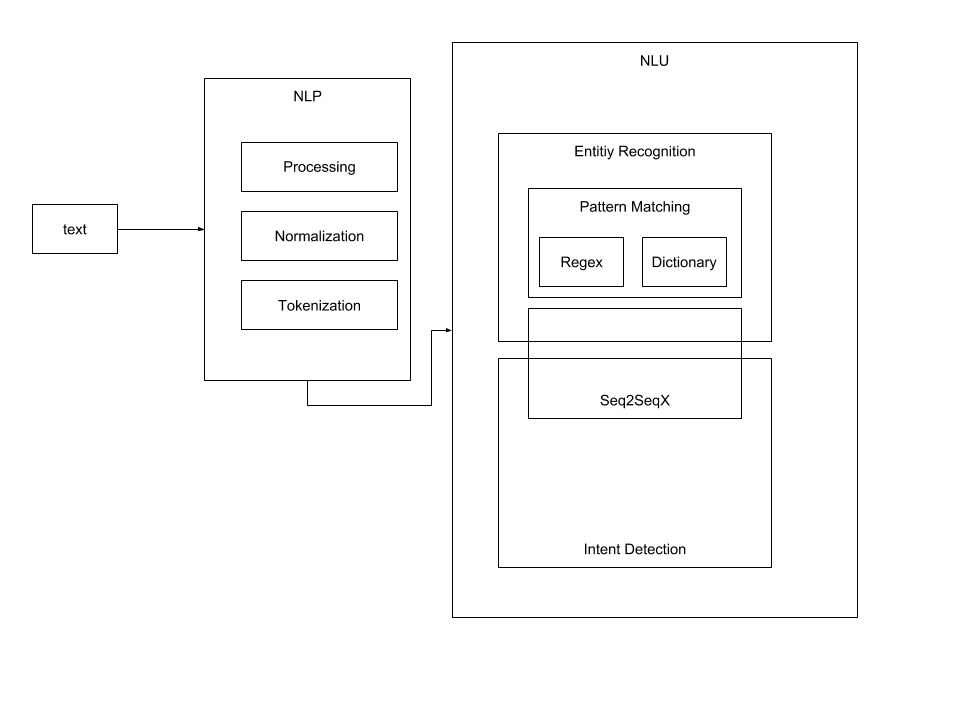
\includegraphics[scale=0.5]{nlu_architecture.png}
	\caption{Arhitectura serviciului de NLU}
	\label{fig:nlu_arch}
\end{figure}

\section{Tehnologii folosite}

Desemnarea tehnologiilor open source folosite ca dependințe poate fi văzută la prima vedere o alegere ușoară, însă este nevoie de o analiză mult mai amănunțită în ceea ce privește specificul proiectului.
Pentru această lucrare am luat în considerare următorii factori: complexitatea de a descrie o rețea neuronală să fie cat mai simpla, dar să reflecte cat mai bine tot procesul matematic din spate, flexibilitatea de a putea jongla cu diferite arhitecturi de rețele. Evident viteza și eficiența cu care aceste biblioteci rulează, dar și dispozitivele pe care ele rulează (CPU/GPU).

\subsection{Python}

Python a fost creat la începutul anilor 1990 de Guido van Rossum la Stichting Mathematisch Centrum (CWI) în Olanda ca un succesor al limbajului, ABC. \cite{pythonhistory}

Python este un limbaj de programare puternic și ușor de învățat. El are structuri de date implementate la un nivel înalt și reprezintă o abordare simplă, dar eficientă a programării orientate pe obiecte. Python are o sintaxa elegantă, ce impune o dactilografiere dinamică, împreună cu natura sa de limbaj interpretat, reprezintă un instrument ideal pentru scripting și dezvoltarea rapidă a aplicațiilor în multe domenii, pe majoritatea platformelor.

Interpretorul Python și biblioteca standard extinsă sunt disponibile gratuit în format sursă sau binar pentru toate platformele majore pe site-ul Web Python. În același site sunt conținute, de asemenea, distribuții și indicii pentru mai multe module, programe, instrumente și documentație suplimentară.

Interpretorul Python este ușor de extins cu noi funcții și tipuri de date implementate în C sau C++ (sau alte limbaje apelabile din C). Python este de asemenea potrivit ca o extensie pentru aplicații personalizate.
\cite{python_tutorial}

\subsection{Numpy}

Numpy este un acronim pentru "Numeric Python" sau "Numerical Python". El este un pachet fundamental pentru calculul științific in Python, ce furnizează funcții precompilate care se execută rapid cu scopul de a efectua operațiile matematice de rutină.  Mai mult decât atât, NumPy îmbogățește limbajul de programare cu structuri puternice de date pentru calculul eficient de vectori si matrice, implementarea sa suportând chiar și dimensiuni uriașe.

SciPy (Scientific Python) este adesea menționat atunci când vine vorba de NumPy. SciPy extinde capabilitățile NumPy cu alte funcții utile pentru minimizare, regresie, transformate Fourier și multe altele.

Atât NumPy și SciPy nu sunt de obicei instalate în mod implicit. NumPy trebuie să fie instalat înainte de a instala SciPy. 

NumPy se bazează pe două module anterioare Python care se ocupă cu matrice. Unul dintre acestea este Numeric. Numeric este ca NumPy un modul Python pentru înaltă performanță de calcul numeric, dar este învechit în zilele noastre. Un alt predecesor al NumPy este Numarray, care este o rescriere completă a modulului Numeric, dar este învechit de asemenea. NumPy este o fuziune a celor două, adică este construit pe codul lui Numeric dar cu caracteristicile lui Numarray.

\subsection{PyTorch}

% todo de citat sursa din https://pytorch.org/tutorials/beginner/blitz/autograd_tutorial.html

PyTorch este o bibliotecă software ce oferă un cadru de lucru cu algoritmi de invățare automată. Se prezintă ca o variantă de Numpy care poate rula pe placa video, având tot odată și capacitatea de autodiferențiere atunci când este nevoie să antrenăm, spre exemplu folosind metoda gradientului descendent.

\textbf{Diferențiere Automată}

Componenta cheie a rețelelor neuronale din PyTorch este pachetul \textit{autograd}. El oferă diferențierea automată pentru toate operațiile cu \textit{tensori}. Este un cadru de definire a operațiilor (forward dar și backward) la momentul execuției, ceea ce înseamnă că pasul de backpropagation este definit de modul în care este rulat codul.

\textbf{Tensor}

\textit{torch.Tensor} este clasa centrală a pachetului. Dacă se setează atributul \texttt{.requires\_grad} ca  \texttt{True}, se va începe urmărirea tuturor operațiilor în care acesta intervine. După ce se termină calculul, se poate apela \texttt{ backward()} pentru a calcula automat toate derivatele, iar gradientul pentru acest tensor va fi acumulat în atributul \texttt{.grad}.

Pentru a opri tensorul din istoricul de urmărire, se apelează \texttt{.detach()} care detașează tensorul de istoricul de calcul și care împiedica urmărirea viitoarelor calcule.

Mai există încă o clasă care este foarte importantă pentru implementarea autodiferențierii - și anume \textit{Function}.

Tensorul și funcția sunt interconectate și construiesc un graf aciclic, care codifică un istoric complet al calculelor. Fiecare tensor are un atribut  \texttt{.grad\_fn} care se referă la o funcție care a creat tensorul (cu excepția tensorurilor creați de utilizator unde - \texttt{.grad\_fn = None}).
	
	\chapter{Concluzii}

Cele profunde concluzii
	
	\bibliography{bibliografie}
	
	\fancyhf{}
	
	\rfoot{\thepage}
	
	\renewcommand{\thesection}{} % nu numeroteaza anexele
	\addcontentsline{toc}{section}{Anexe} % adauga Anexe in Cuprins
	%%% ************************************************************************* %% apendix.tex \ \\ 
\vspace{1.5cm} 
\textbf{\Huge Anexe}\\ 
\vspace{1.5cm}

\pagenumbering{arabic} \setcounter{page}{1}

\large{Ontologie pentru ATIS}
\lstinputlisting[language=json, caption={Ontologie pentru ATIS}, label={lst:ontologie-atis}]{cod/atis_ontology.json}

\newpage
\large{Structura dialogului pentru ATIS}
\lstinputlisting[language=json, caption={Structura dialogului pentru ATIS}, label={lst:dialog-str-atis}]{cod/atis_dialog_knowledge.json}

\large{Exemplu de răspuns al serviciului de NLU}
\lstinputlisting[language=json, caption={Exemplu de răspuns al serviciului de NLU}, label={lst:rsp}]{cod/rsp.json} % afiseaza anexele

\end{document}
